\chapter{Implementación}

La implementación del software se ha dividido en hitos. Estos han sido definidos en Github
y cada uno de ellos contiene un grupo de \textit{issues} que se corresponden con las distintas
mejoras que se han ido incorporando al software a lo largo de su desarrollo.

\section{Toma de decisiones}

\subsection{Elección MTD para servidor web}
Donde el único criterio a tener en cuenta es el consumo de recursos.
Los candidatos para la elección son: MTD CBITS, DARE, DIM, MASS y la implementación de Philip Tibom y Max Buck\cite{MTD-gotemburgo}(K8s).

Como DARE, DIM y MASS son sucesiones de la misma implementación con mejoras en cada una de ellas (como se muestra en el estado del arte) nos quedamos con MASS entre estos tres.
MTD CBITS y K8s son implementaciones de codigo abierto que aportan la solución a escenario cloud/distribuidos, pero para implementarlos en un único servidor supondrían mucha sobrecarga de infraestructura para poder utilizarlo. Por ejemplo para K8s, MTD CBITS y MASS tendríamos que hacer el despliegue en el mismo servidor desde el que manejaríamos el MTD, la diferencia entre K8s, MTD CBITS y MASS es que los dos primeros necesitan la infraestructura de despliegue y de nodo (Kubeadm+Minikube el primero y Puppet+Openstack el segundo) versus MASS (Docker+Firewalld). 

Por lo que atendiendo al consumo de recursos se selecciona el MASS.

\subsection{Gestor de dependencias}
Los criterios para elegir el gestor de dependencias, de mayor a menor prioridad, han sido:
\begin{enumerate}
    \item Soporte pyproject.toml (Ajustandose al PEP 518\cite{pep-pyproject}).
    \item Creación de entornos virtuales/gestión las dependencias de forma local.
    \item Rendimiento.
\end{enumerate}

Donde se van a evaluar los siguientes gestores de dependencias: \textit{Pipenv, Poetry, Hatch, PDM, Conda, Mamba, Pixi, Rye, Miniconda y Micromamba}

\begin{table}[H]
    \centering
    \begin{adjustbox}{width=\textwidth, totalheight=\textheight, keepaspectratio}
        \begin{tabular}{|c|c|c|c|c|c|c|c|c|c|c|c|c|}
            \hline
            Requisitos & Pipenv & Poetry & Hatch & PDM & Conda & Mamba & Pixi & Rye & Pip & Pip-tools & Miniconda & Micromamba\\
            \hline
            Pyproject.toml & \checkmark & \checkmark & \checkmark & \checkmark & \ding{55} & \ding{55} & \ding{55} & \checkmark & \ding{55} & \ding{55} & \ding{55} & \ding{55} \\
            Entornos virtuales & \checkmark & \checkmark & \checkmark & \checkmark & \checkmark & \checkmark & \checkmark & \checkmark & \ding{55} & \ding{55}  & \checkmark & \checkmark \\
            \hline
        \end{tabular}
    \end{adjustbox}
    \caption{Comparativa entre gestores de dependencias.}
\end{table}

Pip y pip-tools, no gestionan entornos virtuales, el resto de opciones si lo hace. Conda, mamba y sus versiones lite no tienen {\tt pyproject.toml}, en cuanto a pixi, este está basado sobre conda, pero genera en el directorio de trabajo su pixi.lock y pixi.toml, el cual no cumple con el estándar de pyproject.toml.

Para evaluar su rendimiento nos basaremos en diferentes benchmarks\cite{pm-benchmark-shootout}. Donde observamos que poetry es el más rápido en realizar la instalación desde un lockfile, creación de este y en añadir un paquete. Además es el segundo en actualizar los paquetes. Sin embargo es el que más tarda en ser instalado. Ya que el gestor de dependencias será instalado una sola vez, vamos a priorizar los otros benchmarks. Por lo que tenemos a poetry como ganador ante PDM y pipenv.

Debido a que no se ha encontrado ningún benchmark sobre Hatch y Rye (este además de que está en un estado experimental), se utilizará poetry como gestor de dependencias.

\subsection{Gestor de tareas}
Los criterios para elegir el gestor de tareas, de mayor a menor prioridad, han sido:
\begin{enumerate}
    \item Curva de aprendizaje.
    \item Ficheros de configuración.
\end{enumerate}

Donde se van a evaluar los siguientes gestores de tareas: \textit{Poethepoet, Pypyr, Invoke, Doit, Pytask}

\begin{table}[H]
    \centering
    \begin{adjustbox}{width=\textwidth, totalheight=\textheight, keepaspectratio}
        \begin{tabular}{|c|c|c|c|c|c|}
        \hline
        Requisitos & Poethepoet & Pypyr & Invoke & Doit & Pytask\\
        \hline
        Curva de aprendizaje & Fácil & Difícil & Medio & Medio & Medio \\
        Ficheros de configuración & pyproject.toml & pipelines/*.yml + .py & tasks.py & dodo.py & task\_*.py \\
        \hline
        \end{tabular}
    \end{adjustbox}
      \caption{Comparativa entre gestores de tareas.}
\end{table}

De las opciones anteriores, poethepoet es el que menos deuda técnica aporta al proyecto, ya que además de permitir funciones en Python como invoke, doit y pytask, permite utilizar shell, comandos y expresiones en Python directamente. Sumando que utiliza el fichero de configuración pyproject.toml, por lo que se evitarían ficheros extra.


\subsection{Test runner}
Los criterios para elegir el \textit{test runner}, de mayor a menor prioridad, han sido:
\begin{enumerate}
    \item Utiliza BDD (Behavior Driven Development).
    \item Estructura de archivos.
    \item Diferentes características.
\end{enumerate}

Donde se van a evaluar las siguientes herramientas: \textit{Pytest, Nose2, Unittest, Green, Behave, Testcontainers, Radish}

\begin{table}[H]
    \centering
    \begin{adjustbox}{width=\textwidth, totalheight=\textheight, keepaspectratio}
        \begin{tabular}{|c|c|c|c|c|c|c|c|}
        \hline
        Requisitos & Pytest & Nose2 & Unittest & Green & Behave & Testcontainers & Radish \\
        \hline
        Utiliza BDD & \checkmark (plugin) & \ding{55} & \ding{55} & \ding{55} & \checkmark & \ding{55} & \checkmark \\
        \hline
        \end{tabular}
    \end{adjustbox}
      \caption{1ª Comparativa entre gestores de tareas.}
\end{table}

Se descartan todas excepto Pytest, Behave y Radish.

La estructura de archivos entre estos apenas varía, todos utilizan \textit{steps}, \textit{features} y un fichero \textit{.ini} (el cual puede ser utilizado para cambiar la estructura).

En este punto los tres son válidos en el proyecto, sin embargo, vamos a comparar algunas características para seleccionar uno:

\begin{itemize}
    \item Paralelismo: Behave no tiene paralelismo nativo (y el plugin que lo soportaba esta deprecated), mientras que Radish lo soporta de forma nativa y Pytest con un plugin (pytest-xdist).
    \item Escenario como precondición: Radish permite que para ejecutarse un escenario se tenga que cumplir otro previamente.
    \item Bucle de escenario: Radish permite ejecutar escenarios en bucle.
    \item Declaración explícita de escenarios: Pytest necesita que en el fichero \textit{steps} se declare explícitamente el escenario.
    \begin{table}[H]
        \centering
        \begin{adjustbox}{width=\textwidth, totalheight=\textheight, keepaspectratio}
            \begin{tabular}{|c|c|c|c|}
            \hline
            Otras características & Pytest & Behave & Radish \\
            \hline
            Dependencias & 11 & 4 & 9 \\
            \hline
            Tamaño & 1.25 MB & 982 KB & 1.89 MB \\
            \hline
            Forks (Github) & 206 & 679 & 48 \\
            \hline
            Stars (Github) & 1.2 K & 3 K & 176 \\
            \hline
            Snyk advisor  & 91 & 71* & 87 \\
            \hline
            \end{tabular}
        \end{adjustbox}
            \caption{2ª Comparativa entre gestores de tareas.}
    \end{table}
\end{itemize}


En esta comparativa se puede ver que Pytest se queda un poco atrás en la facilidad de uso de BDD, mientras que Radish es el que tiene más funcionalidades. Sin embargo estas funcionalidades, como el paralelismo, no se aplicarán a este proyecto, ya que los test modificarán iptables de la máquina donde se ejecute y levantará contenedores, aunque estas tareas podrían ser paralelizables, debido a su complejidad no se realizarán. Otra funcionalidad como los bucles de escenarios no será necesario y los escenarios como precondición podrían ser útiles en otro contexto, ya que este se podría utilizar para comprobar que el docker está corriendo correctamente, pero esto se adaptaría mejor en el \textit{setup} y \textit{teardown} (utilizando menos recursos), por lo que, aunque Radish brinda más funcionalidades, difícilmente serán adaptables a este proyecto, por lo que se va a utilizar Behave el cual cumple con los requisitos necesarios, es el que añade menos dependencias, es el más ligero y cuenta con mayor comunidad (dentro de BDD). Aunque este es marcado en Snyk advisor\cite{snyk} como inactivo, no lo es, ya que este utiliza la última versión en Pypi, la cual salió en 2018, sin embargo el proyecto se ha seguido desarrollando, solo que no cuenta con una nueva versión en Pypi. En Github se puede encontrar su propio versionado y \href{https://behave.readthedocs.io/en/latest/install/#using-the-github-repository}{como descargarlo}.


\subsection{Librería de aserciones}
Los criterios para elegir la librería de aserciones, de mayor a menor prioridad, han sido:

\begin{enumerate}
    \item Por defecto.
    \item Otras características.
\end{enumerate}

Donde se van a evaluar las siguientes librerías: \textit{Assert, Unittest, PyHamcrest, Pytest, Asserpy, Truth, Matchers, Grappa, Verify}

Se descartarán todos excepto Assert y Unittest, los cuales están incluidos por defecto en Python.

Se utilizará Unittest, ya que aunque no se necesite gran variedad de funcionalidades y se pueda conseguir lo mismo con ambas, Unittest permitirá no tener que escribir explícitamente los fallos (lo cual sería más necesario si no se utilizase un BDD) y usar una función autodescriptiva, consiguiendo una mayor legibilidad.

\subsection{Imagen OCI para los servidores}
El MTD deberá de rotar entre dos servidores, esto se llevará a cabo rotando dos contenedores Docker, uno que tendrá un servidor Nginx y otro uno Apache, está deberá ser la única diferencia sustancial entre ambos, ya que deberán de tener el mismo SO y configuración (dentro de lo posible). Por lo que se elegirá una imagen y a partir de esta se creará una para Nginx y otra para Apache. Los criterios para la elección de la imagen han sido los siguientes:

\begin{enumerate}
    \item Peso descarga imagen base (linux/amd64).
    \item Peso imagen montada.
    \item Uso de memoria (reposo).
    \item Seguridad (docker scan Snyk).
\end{enumerate}

Antes de mencionar las imágenes evaluadas se han descartado las imágenes personalizadas que requieran de ficheros estáticos o herramientas externas como Bazel para ser montadas, aquellas que no son oficiales de Docker, editor oficial o \textit{sponsored oss} (para que estas tengan soporte de alguna entidad/persona que implementen mejoras o arreglen bugs) y aquellas orientadas a una implementación de Nginx o Apache, ya que habrá que adaptarlo al otro desde esa imagen. 

Las imágenes a tener en cuenta han sido: \textit{alpine:3.18.4, debian:trixie-20231009, debian:trixie-20231009-slim, phusion/baseimage:jammy-1.0.1, almalinux:9.2, almalinux:9.2-minimal, ubuntu:mantic-20231011, fedora:40, bellsoft/alpaquita-linux-base:stream-musl-231027, bellsoft/alpaquita-linux-base:stream-glibc-231027, gcr.io/distroless/base-debian12:nonroot}

Se utilizarán nombre abreviados de las imágenes a partir de ahora.

\begin{table}[H]
    \centering
    \begin{adjustbox}{width=\textwidth, totalheight=\textheight, keepaspectratio}
        \begin{tabular}{|c|c|c|c|c|c|c|c|c|c|c|c|c|c|c|c|}
        \hline
         Imágenes & alpine & debian & debian-slim & baseimage & almalinux & almalinux-minimal & ubuntu & fedora & alpaquita-musl & alpaquita-glibc & distroless-base \\
        \hline
        Tamaño comprimida & 3.246 MB & 47.210 MB & 28.006 MB & 80.500 MB & 65.054 MB & 31.918 MB & 28.17 MB & 63.100 MB & 3.263 MB & 8.766 MB & 1.012 MB \\
        \hline
        Tamaño montada & 7.34 MB & 116 MB & 75.1 MB & 229 MB & 184 MB & 86.2 MB & 71.2 MB & 185 MB & 7.44 MB & 22.4 MB & 20.7 MB \\
        \hline
        \end{tabular}
    \end{adjustbox}
    \caption{Comparativa del tamaño de las imágenes.}
\end{table}

Donde se descartarán al ocupar bastante espacio:
\begin{enumerate}
    \item Tamaño de la imagen comprimida: debian, baseimage, almalinux, fedora.
    \item Tamaño de la imagen montada: debian-slim, almalinux-minimal, ubuntu.
\end{enumerate}

La elección será entre: alpine, alpaquita-musl, alpaquita-glibc, distroless-base.

\begin{table}[H]
    \centering
    \begin{adjustbox}{width=\textwidth, totalheight=\textheight, keepaspectratio}
        \begin{tabular}{|c|c|c|c|c|}
        \hline
        Imágenes & alpine & alpaquita-musl & alpaquita-glibc & distroless-base \\
        \hline
        Uso de memoria & 5.379 MiB & 5.301 MiB & 5.223 MiB & 5.07 MiB \\
        \hline
        Imágenes & 0 & No info & No info & 9L \\
        \end{tabular}
    \end{adjustbox}
    \caption{Comparativa uso de memoria y CVEs.}
\end{table}

En la comparativa anterior comprobamos que no hay gran diferencia de uso de memoria entre las candidatas. Excepto las alpaquita de las cuales no tenemos información de sus CVEs, y que son descartadas por esto, el resto son seguras.

Aunque no hay mucha diferencia entre ambas alpine es superior, en tres de los cuatro criterios a tener en cuenta, a la imagen \textit{distroless}, por lo que se utilizará una imagen que tenga alpine como punto de partida para ambas imágenes. 

\section{Implementación MTD}
La solución seleccionada fue el MASS, desarrollado por Cimone Le Wright-Hamor. Este MTD se basa en la rotación de dos servidores, uno Apache y otro Nginx, para aumentar la protección de los servidores. El funcionamiento normal del MTD se podría ver como:

\begin{algorithm}
\caption{MASS workflow}\label{mass:algorithm}
    \begin{algorithmic}[1]
        \Function{switch}{}
            \State $container \gets \textsc{contenedor en uso}$
            \If{$container == NGINX$}
                \State Crear contenedor HTTPD
                \State Redirigir el tráfico hacia el puerto del HTTPD
                \State Eliminar el contenedor NGINX
            \Else
                \If{$container == HTTPD$}
                    \State Crear contenedor NGINX
                    \State Redirigir el tráfico hacia el puerto del NGINX
                    \State Eliminar el contenedor HTTPD
                \EndIf
            \EndIf
        \EndFunction

        \Function{start}{rango\_arriba, rango\_abajo, duración}
            \State $SERVER \gets NGINX$
            \While{$tiempo \l duración$}
                \State $tiempo\_espera \gets \textsc{Valor aleatorio}(rango\_arriba , rango\_abajo)$
                \State \textsc{sleep}(tiempo\_espera)
                \State \textsc{switch}\Comment{Rota el servidor en uso}
            \EndWhile
        \EndFunction
    \end{algorithmic}
\end{algorithm}

Donde originalmente tiene esta estructura:
\begin{figure}[H]
    \centering
    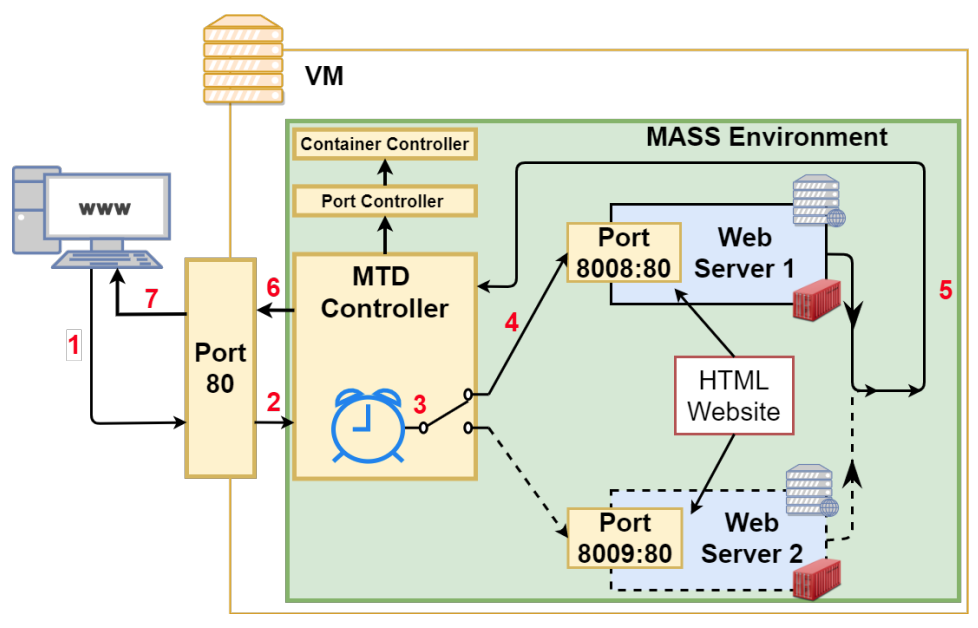
\includegraphics[width=\linewidth]{./imagenes/mass-structure.png}
    \caption{Estructura original del MASS con flujo de tráfico.\cite{MTD-DARE-DIM-MASS}}
\end{figure}

\begin{itemize}
    \item Controlador del MTD: el cual es el encargado de controlar el tiempo y activar el cambio de servidor. Soporta tanto rotación en intervalos fijos como entre un rango de tiempos.
    \item Controlador de contenedores: es el encargado de encender y matar los contenedores con los servidores.
    \item Controlador de puertos: es el encargado de controlar el \textit{firewall} para redirigir el tráfico desde el puerto 80 a el puerto interno del servidor activo (8008 y 8009). 
\end{itemize}

En la implementación realizada se han separado el controlador de contenedores del de puertos, siendo ambos controlados directamente por el controlador del MTD. Esta representación se puede ver en el siguiente diagrama de clases.

\begin{figure}[H]
    \centering
    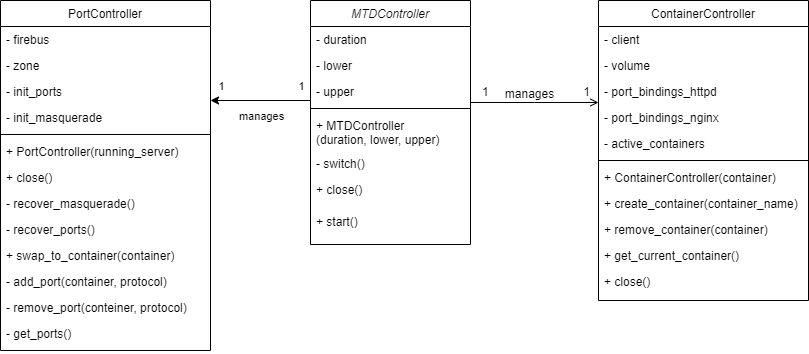
\includegraphics[width=\linewidth]{./imagenes/clases.png}
    \caption{Diagrama de clases de la implementación.}
\end{figure}


\section{Tests}
Para comprobar si la solución se ajusta a los requisitos se han desarrollado los siguientes tests:
\begin{itemize} 
    \item Uso de CPU en reposo: para ver como afecta la rotación de los servidores a el uso normal del servidor. 
    \item Rendimiento: para comprobar cuanta carga de peticiones puede soportar y como afecta al uso de CPU.
    \item Explotación: se ha explotado una vulnerabilidad en uno de los dos servidores para ver si la rotación ayuda a mitigar el tiempo de exposición.
\end{itemize}

